\documentclass[12pt]{article}
\usepackage[english]{babel}
\usepackage{amsmath}
\usepackage{amsthm}
\usepackage{amssymb}
\usepackage{amsfonts}
\title{HDP Notes and Exercise Soultions}
\author{Holden Caulfield}
\newtheorem{theorem}{Theorem}
\newtheorem{remark}{Remark}[theorem]
\newtheorem{ex}{Problem}
\usepackage{enumitem}
\usepackage{graphicx}
\usepackage{tcolorbox}
\usepackage{caption}
\usepackage{xcolor}
\usepackage{tikz}
\tcbuselibrary{skins}
\tcbuselibrary{breakable}
\usepackage{subcaption}
\usepackage{float}

\begin{document}
	\begin{center}
	
		\section{N-gram Language Models}

		\hrule
		\vspace{0.25cm}
		
		\subsection{N-gram Language Modeling \& Perplexity}
		
		\begin{enumerate}[label=(\alph*)]
			\item
			To construct the N-gram models, we need to calculate the conditional distribution over the $n$-th token given the previous $n-1$ tokens. To do so, we count the number of occurrences of the string $x_i,\dots,x_{i+n-1}$ and divide by the number of occurrences of $x_i,\dots,x_{i+n-2}$.
			
			For the Unigram model we basically count the number of occurrences of each word and divide by the sum of all occurrences of all words.
			
			We can see the top 30 most frequent tokens for all 3 models below.
			\begin{figure}[!htbp]
				\centering
				\begin{minipage}[b]{0.45\textwidth}
					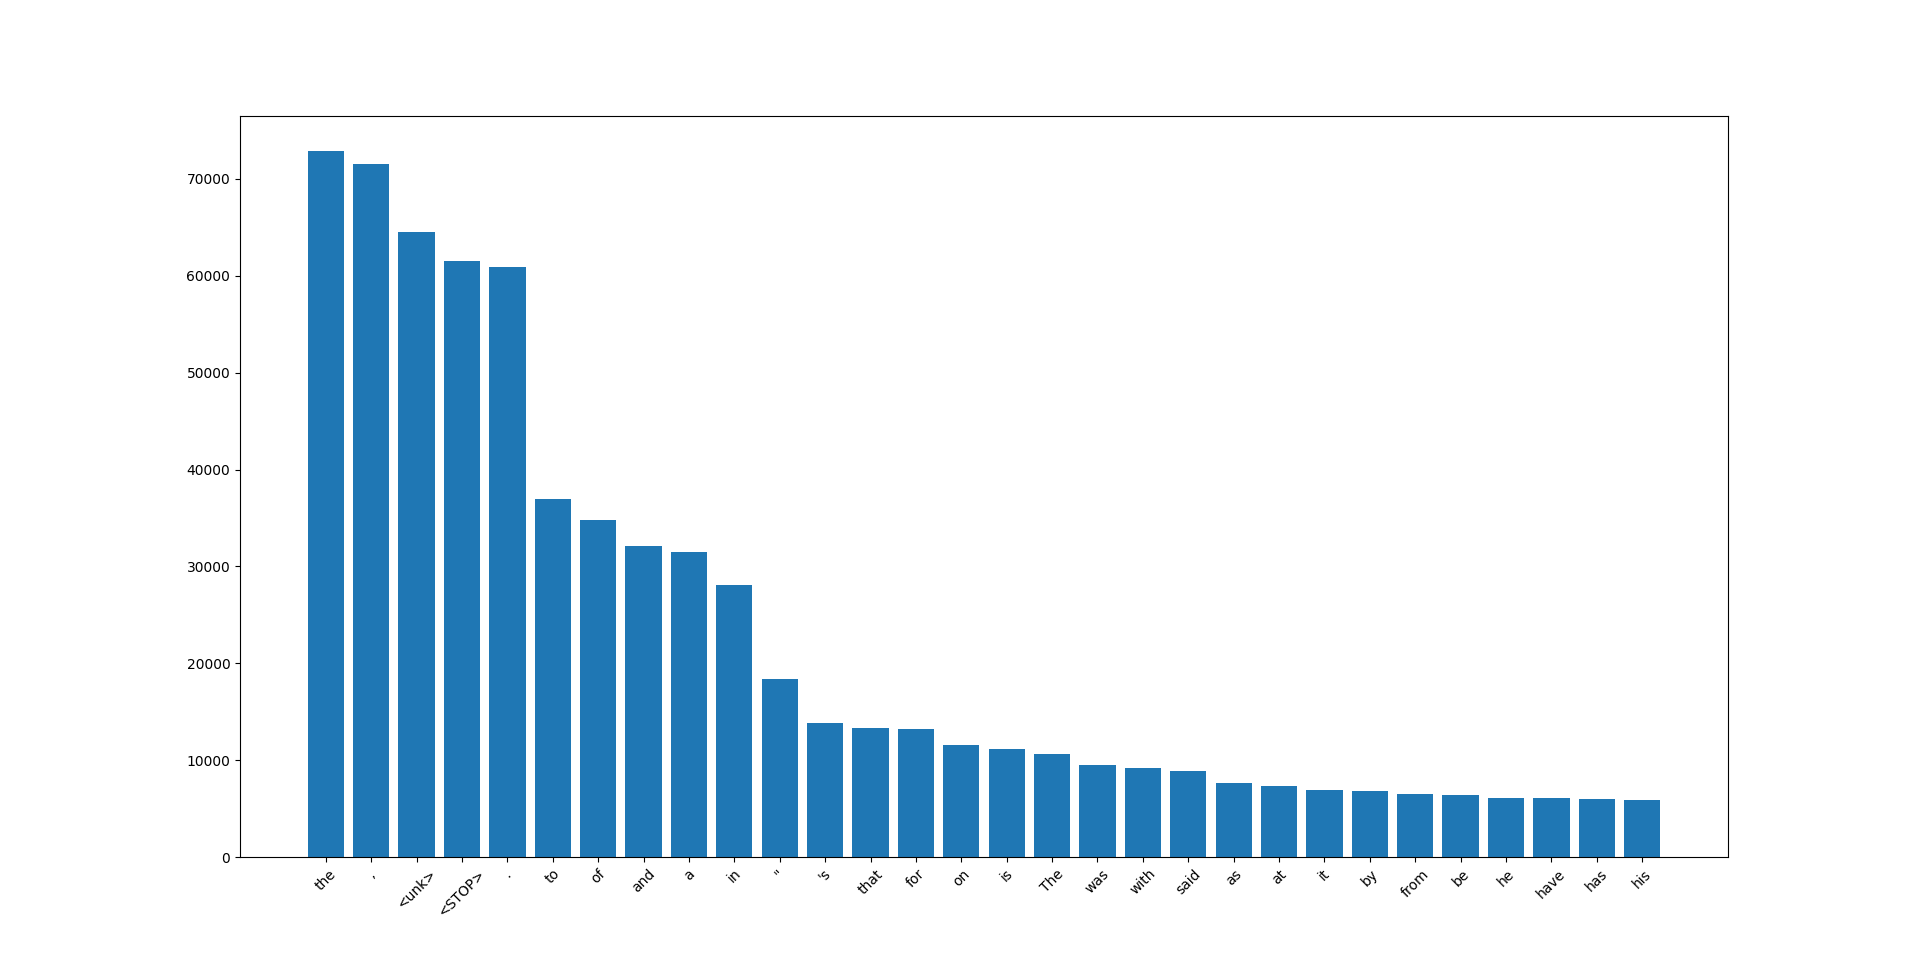
\includegraphics[width=\textwidth]{token_dist.png}
					\caption*{Unigram}
				\end{minipage}
				\hfill
				\begin{minipage}[b]{0.45\textwidth}
					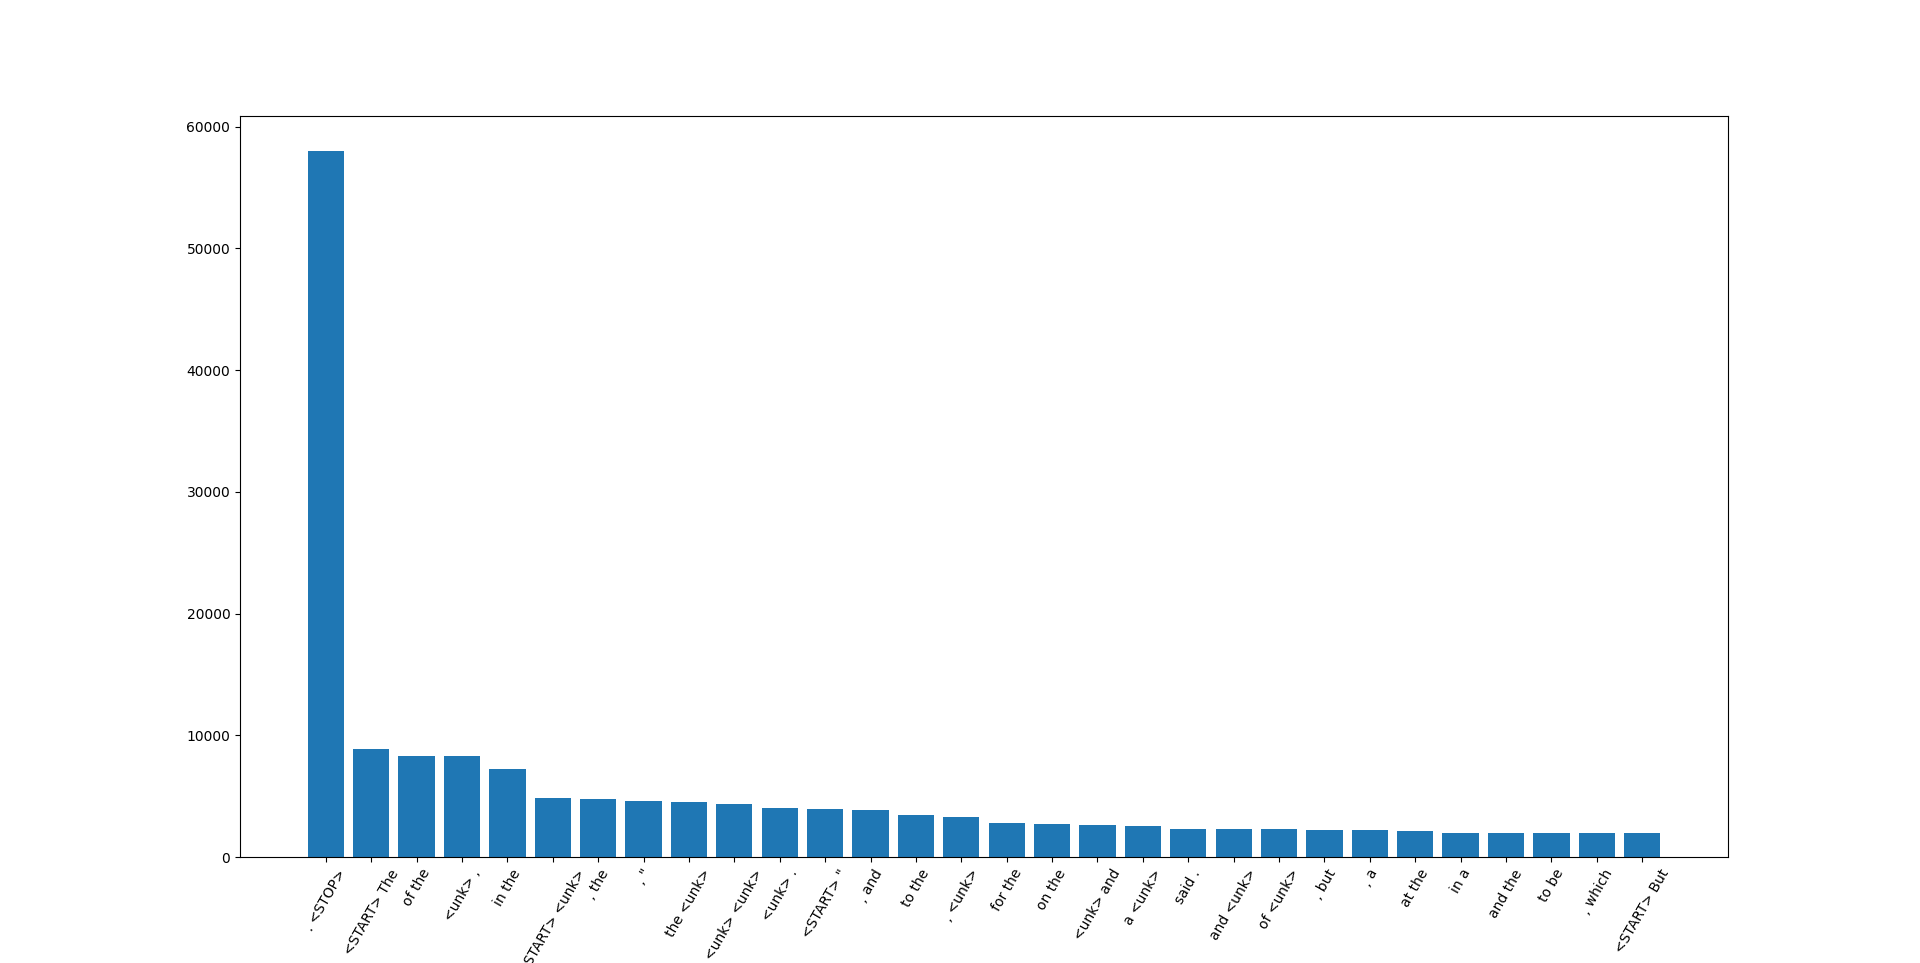
\includegraphics[width=\textwidth]{bigram_dist.png}
					\caption*{Bigram}
				\end{minipage}
				\vskip 1em
				
				\begin{minipage}[b]{0.55\textwidth}
					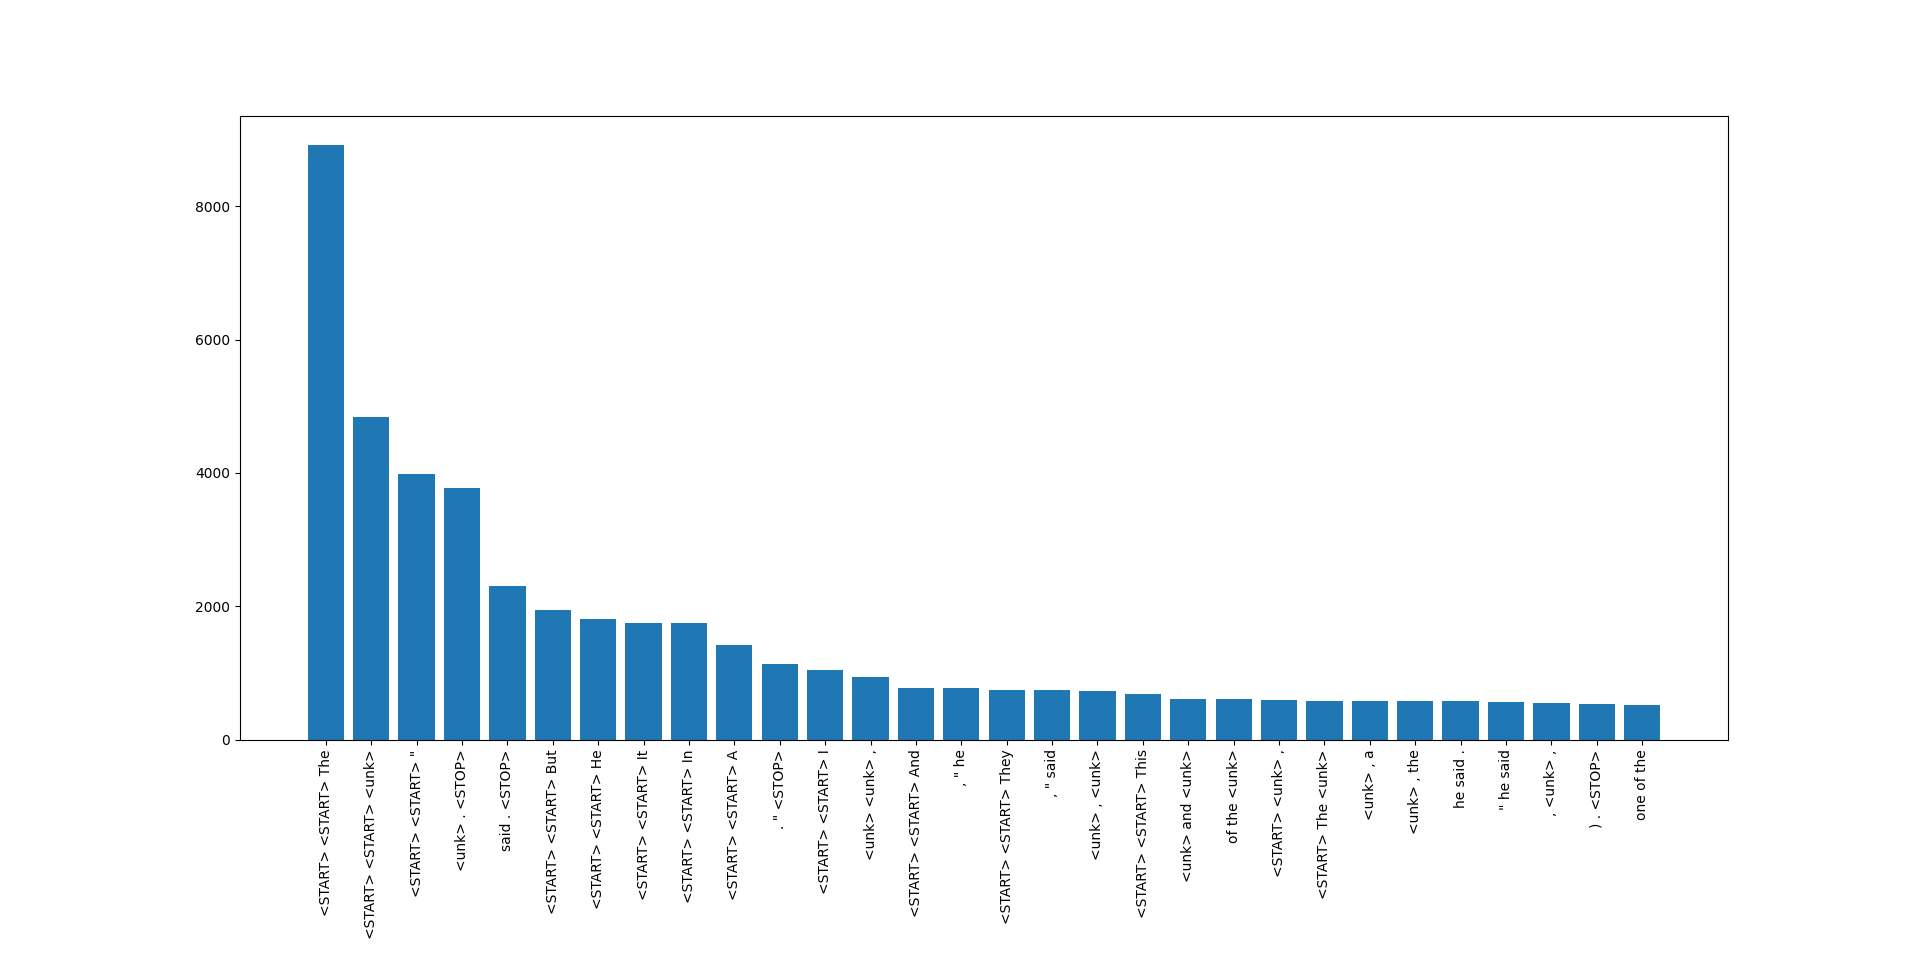
\includegraphics[width=\textwidth]{trigram.png}
					\caption*{Trigram}
				\end{minipage}
				\caption{Top 30 most frequent tokens}
			\end{figure}
			
			\item To calculate the perplexity, we need to calculate the likelihood of each sentence in the given data under the probabilities given by the model, take the geometric mean of its inverse, and then calculate the average over the whole corpus.
			
			There are two things that we need to keep in mind:
			
			\begin{itemize}
				\item Unobserved tokens: to solve this problem, we replace the tokens seen less than 3 times with the special $<$unk$>$ token during training, and replace the unseen tokens with $<$unk$>$ during test time. This would prevent undefined behavior (e.g divide by 0) for the unigram model.But the problem is still unsolved for bigram and trigram models, since there may still be bigrams/trigrams that we have not seen during training. To work around this problem we assume independence for the bigram model i.e. $p(x|y)=p(x)$ and the  Markov assumption for the trigram model i.e. $p(x_{t}|x_{t-1},x_{t-2})=p(x_{t}|x_{t-1})$. With these assumptions, we will no linger witness undefined behavior during perplexity calculation.
				
				\item Conditioning: This problem only applies to bigram and trigram models since they calculate conditional probabilities. To work this problem around, we need to pad each sentence with $n-1$ $<$START$>$ tokens.
			\end{itemize}
			
			\item A potential downside of Laplace smoothing is increasing the perplexity. This lies in the relation between perplexity and entropy:
			\[
			PP(W)=p(w_1,\dots,w_N)^{-\frac{1}{N}}=2^{H(W)}
			\]
			By smoothing, we are giving mass to the unobserved sequences, which could lead to an increase in entropy and thus an increase in perplexity as we will see in the results in section (e).
			
			\item We can see the effect of $k$ in the plots below.
			
			As we can see, trigram has lower perplexity than bigram, but both show the same increasing pattern over k.
			
			\begin{figure}[H]
				\centering
				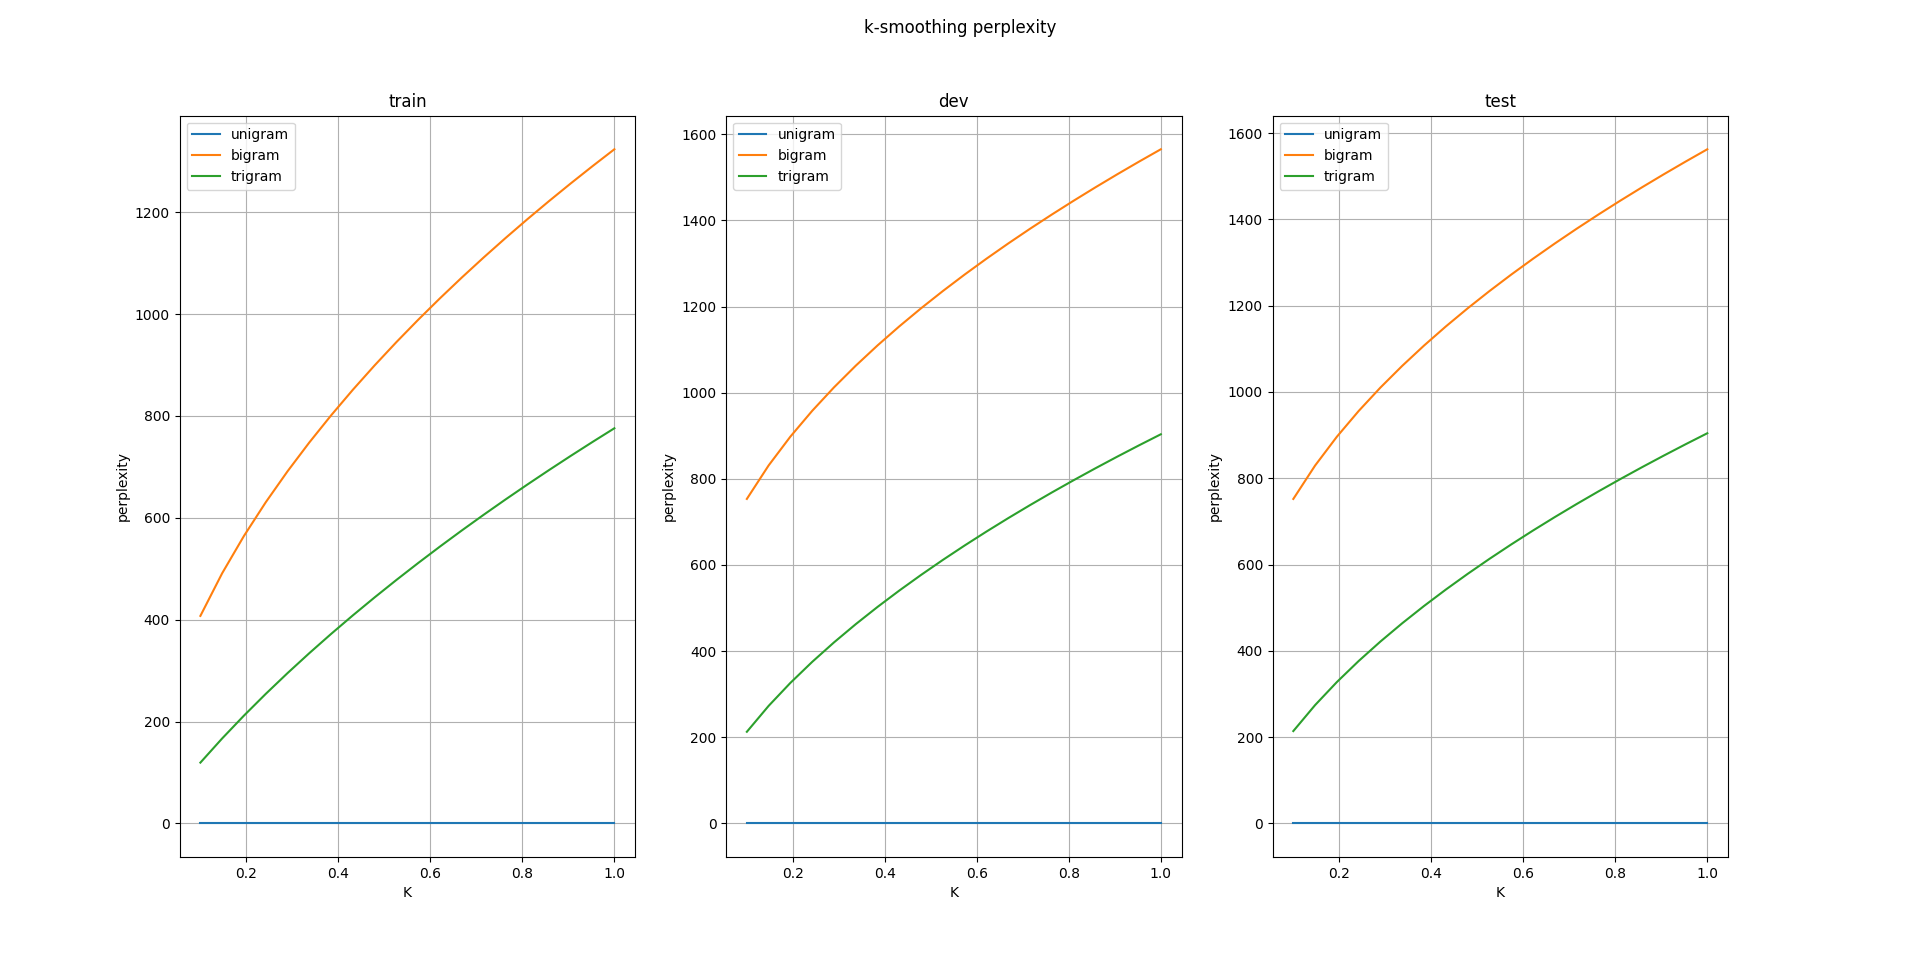
\includegraphics[width=\textwidth]{smooth.png}
				
				\caption{Top 30 most frequent tokens}
			\end{figure}
			
			\item The results are given in the table below.
			
			As wee can see, increasing context-length leads to perplexity improvement without smoothing.
			
			As discussed in section (c), smoothing would increase perplexity; as we can see in the table.
			
			\begin{table}[H]
				\centering
				\begin{tabular}{|c|c|c|}
					\hline
					&\multicolumn{1}{c|}{\textbf{Smoothing}}&\multicolumn{1}{c|}{\textbf{No Smoothing}} \\
					\hline
					& \textbf{Train}: $2.53e-05$ & \textbf{Train}: $1080.36$  \\
					\textbf{Unigram} & \textbf{Dev}: $2.5e-05$ & \textbf{Dev}: $985.55$ \\
					& \textbf{Test}: $2.5e-05$ & \textbf{Test}: $998.72$ \\
					\hline
					
					& \textbf{Train}: 1323.57  & \textbf{Train}: 74.06\\
					\textbf{Bigram} & \textbf{Dev}: 1565.41 & \textbf{Dev}: 193.59 \\
					& \textbf{Test}: 1562.44 & \textbf{Test}: 194.49 \\
					\hline
					
					& \textbf{Train}: 775.76 & \textbf{Train}: 8.37 \\
					\textbf{Trigram} & \textbf{Dev}: 903.56 & \textbf{Dev}: 132.22 \\
					& \textbf{Test}: 904.22 & \textbf{Test}: 132.14 \\
					\hline
				\end{tabular}
				\caption{n-gram perplexity}
			\end{table}
		
		\newpage
				\subsection{Interpolation}
				\begin{enumerate}
				\item The results are shown in the table below with the best result in boldface. My strategy for finding suitable lambdas was to try giving more attention to more/less recent tokens to see how it would affect perplexity. (note that these results come from the dev set)
			\begin{table}[H]
				\centering
				\begin{tabular}{|l|l|l|l|}
					\hline
					$\lambda_1$ & $\lambda_2$ & $\lambda_3$ & \textbf{perplexity} \\ \hline
					0.33 & 0.33 & 0.33 & 151.89 \\ \hline
					0.6 & 0.3 & 0.1 & 190.79 \\ \hline
					0.3 & 0.6 & 0.1 & 157.67 \\ \hline
					0.3 & 0.1 & 0.6 & 148.6 \\ \hline
					\textbf{0.1} & \textbf{0.3} & \textbf{0.6} & \textbf{134.4} \\ \hline
					0.6 & 0.1 & 0.3 & 184.38 \\ \hline
				\end{tabular}
			\end{table}
		\item The same set that achieved the lowest perplexity on the dev set, achieves the lowest perplexity on the test set with a perplexity of $134.48$.
		
		\item Halving the the training data leads the an increase in perplexity, this is because reducing sample size would make our estimates more biased, hence it would decrease the performance on unseen data as can be seen in the table below 
		\begin{table}[!ht]
			\centering
			\begin{tabular}{|l|l|l|l|}
				\hline
				$\lambda_1$ & $\lambda_2$ & $\lambda_3$ & perplexity \\ \hline
				0.33 & 0.33 & 0.33 & 167.99 \\ \hline
				0.6 & 0.3 & 0.1 & 206.39 \\ \hline
				0.3 & 0.6 & 0.1 & 172.1 \\ \hline
				0.3 & 0.1 & 0.6 & 165.88 \\ \hline
				0.1 & 0.3 & 0.6 & 150.44 \\ \hline
				0.6 & 0.1 & 0.3 & 202.25 \\ \hline
			\end{tabular}
		\end{table}
		
	
	\item Setting a threshold of $\le5$ would yield a lower entropy compared to $\le1$, thus it would give lower perplexity compared to $\le1$ under similar conditions as can be seen below.
	
	\begin{table}[H]
		\centering
		\begin{tabular}{|l|l|l|l|}
			\hline
			$\lambda_1$ & $\lambda_2$ & $\lambda_3$ & perplexity \\ \hline
			0.33 & 0.33 & 0.33 & 169.86 \\ \hline
			0.6 & 0.3 & 0.1 & 212.63 \\ \hline
			0.3 & 0.6 & 0.1 & 175.89 \\ \hline
			0.3 & 0.1 & 0.6 & 166.54 \\ \hline
			0.1 & 0.3 & 0.6 & 150.52 \\ \hline
			0.6 & 0.1 & 0.3 & 206.07 \\ \hline
		\end{tabular}
	\caption{threshold=1}
	\end{table}

\begin{table}[!ht]
	\centering
	\begin{tabular}{|l|l|l|l|}
		\hline
		$\lambda_1$ & $\lambda_2$ & $\lambda_3$ & perplexity \\ \hline
		0.33 & 0.33 & 0.33 & 123.75 \\ \hline
		0.6 & 0.3 & 0.1 & 156.06 \\ \hline
		0.3 & 0.6 & 0.1 & 129.18 \\ \hline
		0.3 & 0.1 & 0.6 & 120.57 \\ \hline
		0.1 & 0.3 & 0.6 & 109.51 \\ \hline
		0.6 & 0.1 & 0.3 & 149.94 \\ \hline
	\end{tabular}
\caption{threshold=5}
\end{table}
	
	\newpage
	
	\section{Byte-Pair Encoding (BPE)}
\begin{enumerate}[label=(\alph*)]
	\item The training data is 147408 tokens long under the final vocab. The final vocab size is 4873.
	below we can see the change in vocab size and corpus length over the first 100 iterations.
	\begin{figure}[H]
		\centering
		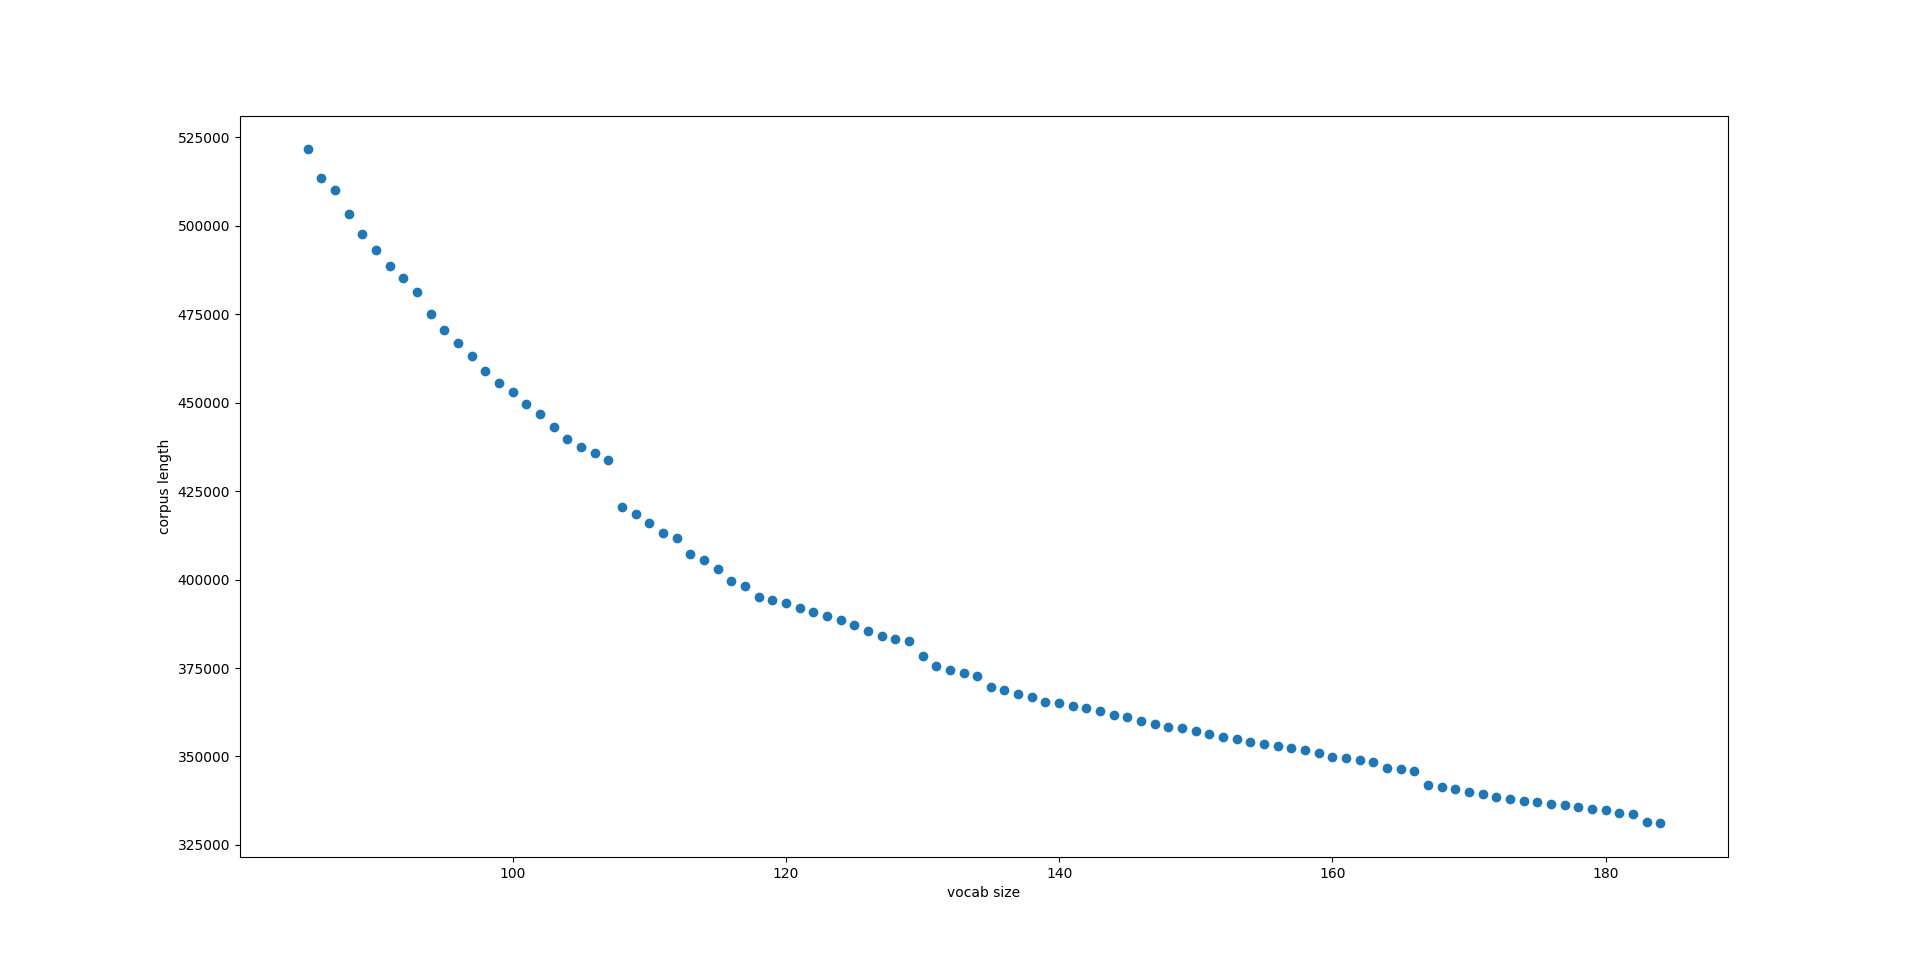
\includegraphics[width=0.55\textwidth]{loop.png}
		
	\end{figure} 
	\item An advantage is that it is simpler to implement than BPE, and a potential downside is that the number of tokens would be much more compared to BPE, which means that it is less efficient in terms of memory usage.
	

	\item We end up with 3265 tokens in total. No Issues witnessed regarding the words not in the training set. A potential scenario that may cause issues is when we train the encoder on one domain and apply it to another one e.g. training on English text and applying to Japanese could cause problems, since the two differ in alphabets.
\end{enumerate}
		
		\end{enumerate}
	\end{enumerate}
\newpage
\section{WordPiece}
\begin{enumerate}[label=(\alph*)]
\item We can see the plot over the first 100 iterations below. The final vocab size is 4085, and the final length of the training data is 368607.
\begin{figure}[H]
	\centering
	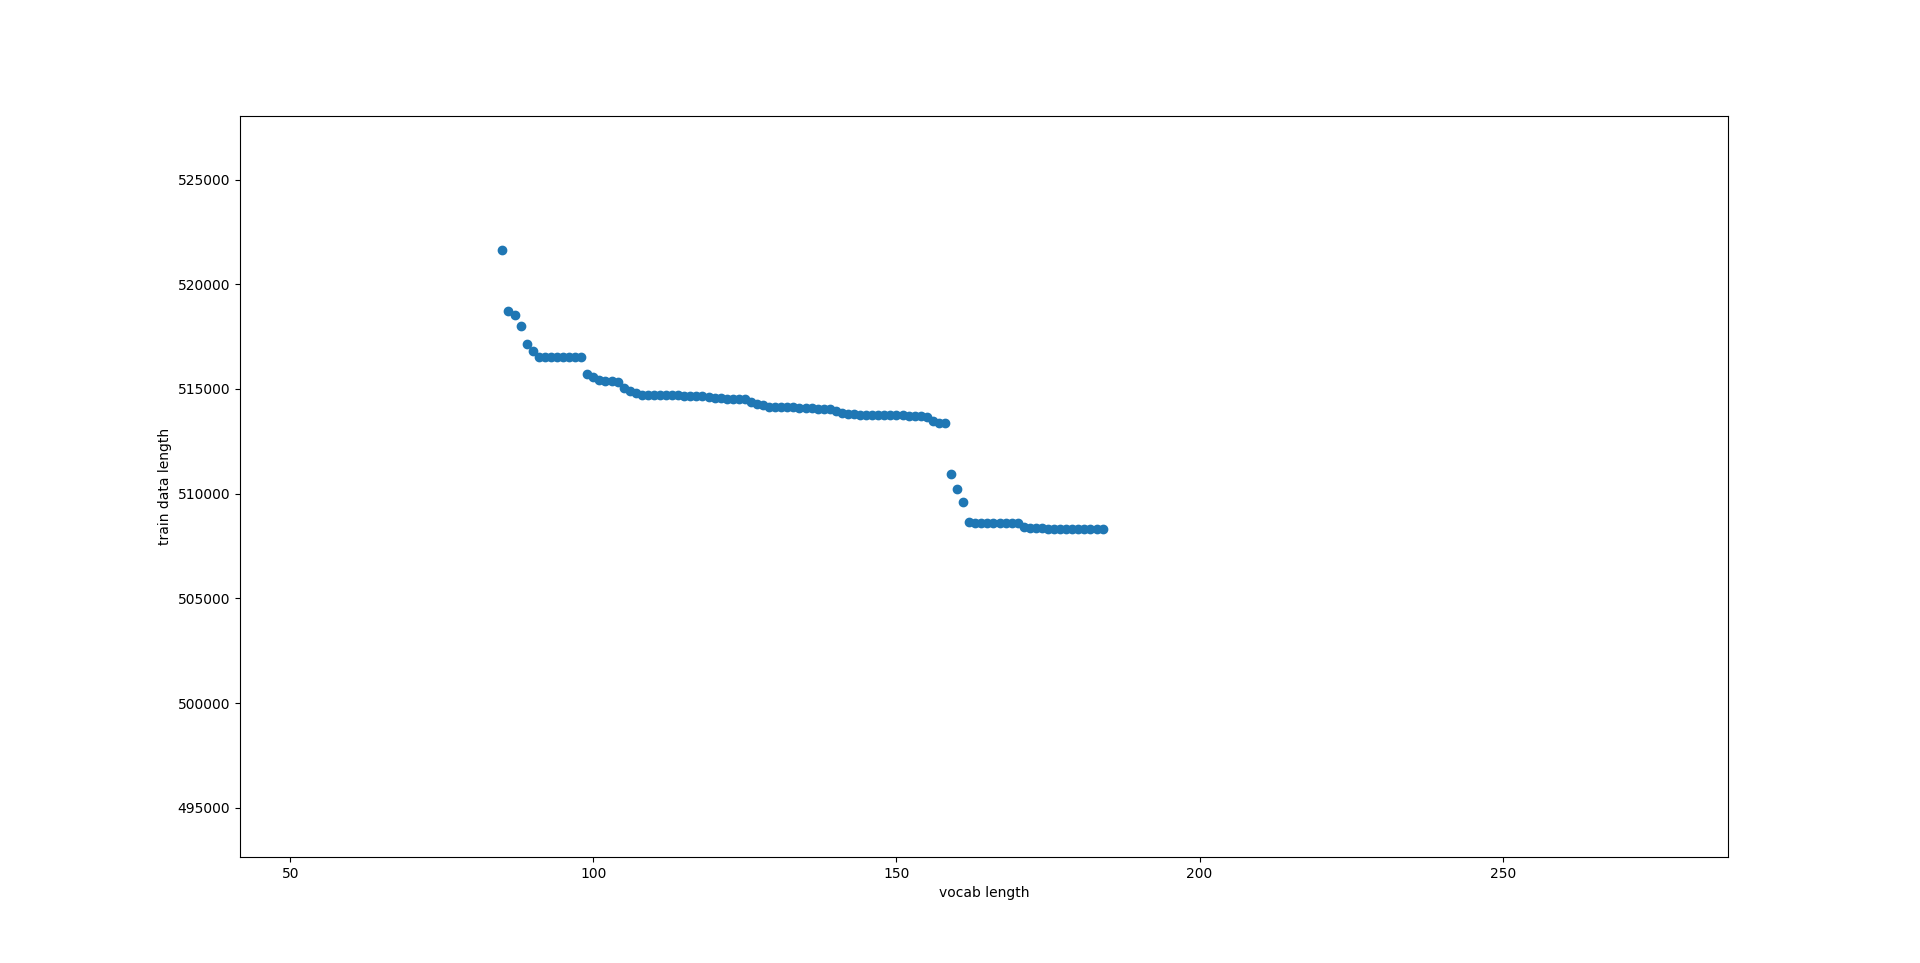
\includegraphics[width=0.5\textwidth]{wp.png}
\end{figure}
\item The test data is 89374 tokens long.The tokenized sequences of the sentences are as follows:
\vspace{0.5cm} \\
\sloppy
['A', 'n', 'a', 'l', 'y', 's', 't', 's', ' ', 'we', 're', ' ', 'e', 'x', 'pecting', ' ', 't', 'he', ' ', 'o', 'p', 'posit', 'e', ',', ' ', 'a', ' ', 'de', 'e', 'pen', 'ing', ' ', 'o', 'f', ' ', 't', 'he', ' ', 'de', 'ficit', '.']
\fussy
\vspace{0.5cm} \\
\sloppy
['F', 'i', 've', ' ', 'minutes', ' ', 'la', 'ter', ',', ' ', 'a', ' ', 's', 'e', 'c', 'on', 'd', ' ', 'person', ' ', 'a', 'r', 'ri', 've', 'd', ',', ' ', 'a', 'ge', 'd', ' ', 'a', 'ro', 'u', 'n', 'd', ' ', 't', 'hi', 'r', 't', 'y', ',', ' ', 'w', 'i', 't', 'h', ' ', 'k', 'n', 'i', 'fe', ' ', 'wounds', '.']
\fussy
\item When applied to the training data, BPE gave us 147408 tokens, while WordPiece gave us more than 300000 tokens, which implies that BPE is more efficient in that regard. At inference time, it took BPE $0.02$ seconds to be applied on the test data, while it took WordPiece more than 5 seconds.

\newpage
\section{Open-ended Exploration for Tokenization}
\begin{enumerate}
	\item Our sample sentence is:
	
	 "If you get on the side where all the hot-shots are, then it’s a game, all right—I’ll admit that. But if you get on the other side, where there aren’t any hot-shots, then what’s a game about it? Nothing. No game.
	
	-Holden Caulfield"
	
	We use Claude and Llama3 for tokenization, and we pick Persian as the second language.
	
\begin{table}[!ht]
	\centering
	\begin{tabular}{|l|l|l|}
		\hline
		 &English& Persian \\ \hline
		Claude & 70 & 165  \\ \hline
		Llama3 & 63 & 65 \\ \hline
		
		
	\end{tabular}

	\caption{Number of tokens}

\end{table}
		The translation was done by myself since Persian is my mother tongue.
		
		\item Another scenario which could lead to such a problem is when a single word in one language needs more words of another language to be described. Take the word "wimpy" as an example, which is a single word in English, but there is a Persian synonym with 4 words.
		
		\item If not handled well, the time it takes for the model to tokenize a given text would vary accross different languages, which means that it could possibly take much longer for some languages, in which case we wouldn't be able to attract the speakers of those languages because of the poor user experience.
		
		\item Although it may not be the best one, but one possible solution could be training tokenizers tailored to each specific language, in which way our tokenizers would be more efficient since they are optimized for that specific language.
\end{enumerate}
\end{enumerate}
\end{center}
\end{document}